\chapter{Sampling on Hadoop} % (fold)
\label{cha:sample}

In this chapter we present a method for data sampling on Hadoop that is basad
in a random algorithm.

\section{Motivation for sampling}

One important aspect in Big Data environments is the vast amount of data,
that is the main barrier to find a job configuration which best suits to the
current state of the cluster~\cite{Chen:2012}. BAs allow to create new configurations,
but these configurations must be tested in order to select which is the best for
the job at a given moment. Moreover, the volatility of the computing nodes (joining and leaving),
big cluster setups at any time and data volatility, may spoil performance depending
on the configurations setup. 

Therefore, caused by the volatility of the cluster and the data, the job configuration
may become deprecated and needs to be reviewed constantly. The review process consists
in choosing a new configuration and testing it in order to analyse the performance.
But the testing cannot be done on the entire data because may be time consuming.

The main question is: {\it How to test job configurations generated by BAs?} One possible
answer is to run the job on data sampling, because the sampling in a database is
a essential step to improve the response time, moreover run the job on all data
stored would spend a lot of time and also would be impracticable due to larger number
of intermediate configurations generated by the algorithm.

\section{Challenge for data sampling in Big Data environments}

On Big Data environments there are several aspects involving distributed computing
and storage. For data sampling the both aspects are relevants and need to be considered.
In this context, the volume of data is the main issue because the data sampling must
be distributed too, otherwise one machine couldn't bear all data storage in the
cluster then make the data sampling. For instance, suppose that one cluster stores
100 terabytes and we want data sampling of 20$\%$, then each node must sample and
store locally. The resulting sample will be 20 terabytes: which one single machine
may not have such storage capacity.

So the resulting data sample must be distributed in the cluster, because it might
be too big to be store on a single machine. After the sample is obtained, jobs
can be run on the sampling. So, as the example would avoid to run the job on 100
terabytes and run just 20 terabytes.

%So the sampling must be done distributed and it must be done without intrusion
%in the Hadoop, because any change done inside of the framework can propagate collateral
%effects due its complexity. Further more to run test regression is a very costly
%activity~\cite{hadoopUnit} and to create unit test cases for the new changes spend
%much time.

The Hadoop has the structure for distributed computing and storage, so a way to 
produce a sample is to utilize the benefits of Hadoop, i.e. taking into consideration
that the data are already distributed. As a consequence, we can build one MapReduce
program to sample data and then benefit from its advantages.

One of the most used data sample techniques is Random Sampling that consists
in selecting a pre-determined amount of data randomly~\cite{randomsampling}.
In the literature there are several others techniques such as Stratified Random Sampling,
which splits data in strata where each element has the same chance of being selected
\cite{de1986sampling}. Another thechnique is Systematic Sampling that consists
in select randomly one element of the population, from this element the next $k$
elements are select in sequence, the number $k$ may be choosen randomly or based
in some criteria. The systematic process continues till the sample is completed~\cite{systematicsampling}.

%has
%one number {\it k} which is chosen randomly or chosen with some criteria, then
%randomly one element is chosen of the population and from this element till the
%next k-esimo elements in sequence are selected to sample~\cite{systematicsampling}.

In the context of big data there are some implementations of data sample. One example
is MonetDB which is a column-oriented database management system designed to hold
data in main-memory and processing distributed of large-scale data~\cite{monetDB}.
This database supports data sample and uses the {\it Algorithm A} which is based on
a random sample method~\cite{monetDB:sampling}.

The {\it Algorithm A} select {\it n} records from a file containing {\it N} records where
$0\le{\it n}\le{\it N}$. For each record that will be inserted in the sample,
it chooses randomly one number {\it V} that is uniformly distributed between 0 and 1.
Based on {\it V, n} and {\it N}, the number {\it s} is calculated. The set of records
{\it S} is then created from {\it s}. This set contains the {\it (s + 1)} first
records of the file. Then one record is chosen from {\it S} and added to the sample.
The records present in {\it S} are skipped in the next interaction~\cite{vitter:1984}.

The {\it Algorithm A} behaves as the stratified random sampling technique. The creation
of the set S can translate to one stratum that contains neighbors records which one
record is chosen.

Hive is another database management system that performs data sampling based on
random methods. Hive was created to manage the data stored on Hadoop, allowing ad-hoc
queries (with are casts to Hadoop MR jobs), data summarization and analysis of
large datasets. Thus, Hive is considered a DW for Hadoop~\cite{hiveWiki}. It samples at
row or block size level. The row level consists in choosing randomly the rows
according with the colunm name. If the column name is not defined, then the entire row
is selected. If it is defined the choice can be done using the Bucketized Table
in which the sample is done only on the buckets that contains
the specified column~\cite{hiveSample}. The block size sample is also done ramdomly
and consists in selecting the blocks that match with the specified block size.

Those sample methods on Hive are based on random sample and handle structured data.
Hive consists storing the Hadoop data as a data warehouse and facilitate
queries submitted by users. Moreover, the clustering by bucket and block size
requires a prior structuring of data, so in the Hive several information about the
data are previously known.

In Hadoop, data are stored in a unstructured manner and this characteristic is the
biggest challenge to develop data sampling methods. According to~\cite{vitter:1985, cloudera, greg, wikipedia:ReservoirSampling}
the challenge with unstructured data stream can be addressed with Reservoir Sampling:
"{\it Say you have a stream of items of large and unknown length that we can only
iterate over once. Create an algorithm that randomly chooses an item from this
stream such that each item is equally likely to be selected.}"

The Reservoir Sampling algorithm is also a random algorithm. It consists in
randomly choosing {\it k} elements from a list {\it L} containing $N$ items.
The length N is either unknown or too large to fit in memory.

To understand the algorithm one example can clarify the idea. Suppose we have one
reservoir sampling of size equal $1$ and we have to get one item such
that all items have the same probability to be choosen.

In the first round when the first item cames the probability is $P(1)^{1}=1$ because
the stream length is $1$ at the moment and we unknow if the stream finished. When
the next element cames (second element), the first element has been holding and
we need to choose continuing hold the first or choosing the second element. So,
the probability to choose the second element is $P(2)=\frac{1}{2}$ because the stream length
is $2$ at the moment. On the other hand, the probability $P(1)^{2}$ continuing hold the
first element is the probability to choose it in the last round multiple by the
probability doesn't choosing the second element, which is $P(1)^{2}=P(1)^{1} \times \overline{P(2)} = 1 \times \left(1-P(2)\right) = 1 \times \left(1 - \frac{1}{2}\right) = 1 \times \frac{1}{2} = \frac{1}{2}$.
So, the probability of the first and the second element in the second round is $\frac{1}{2}$.

In the next round when the third element cames, we need to decide if continue holding
the element chosen in the last round or if we choose the third element. The probability
to choose the third element is $P(3) = \frac{1}{3}$ because the stream length at the moment
is 3. Now, we need to calculate the probability to continue holding the element
chosen in the last round, considering which is the first element, its probatility
in the third round is the probability of it in the second round multiple
by the probability doesn't choosing the third element: $P(1)^{3}=P(1)^{2}\times\overline{P(3)} = \frac{1}{2} \times \left(1-P(3)\right) = \frac{1}{2} \times \left(1 - \frac{1}{3}\right) = \frac{1}{2} \times \frac{2}{3} = \frac{1}{3}$.
So, the probability of the first, second and third element in the third round is
the same, i.e. $\frac{1}{3}$.

In sequence, for the $Nth$ round the probability of all elements is $1/N$. We
can prove such idea by induction:
\\
\\
\\
\\
\begin{itemize}
	\item \emph{Base Case}: $N = 1$.
		\begin{alignat*}{1}
			\texttt{The probability for the first element is $P(1) = \frac{1}{N} = 1$.}
		\end{alignat*}

	\item \emph{Induction Step}: $N > 1$.\\
		\texttt{By the induction hypothesis, the probability for all elements in the\\
				round $N$: $P(1)$ $...$ $P(N)$ $=$ $\frac{1}{N}$.}\\
		\texttt{In the round $N+1$, when the $N+1$ element cames its probability to be chosen is
				$P(N+1) = \frac{1}{N+1}$. Because the stream length is $N+1$ at the moment.}\\
		\texttt{We need to prove that the probability of the all other elements is the same.}
		\texttt{Let's prove the probability of the elements 1 to N in the round $N+1$:}
		\begin{alignat*}{2}
			\texttt{$P($$1$ $to$ $N)$ = }& \texttt{(the probability of the all elements in the round $N$)}\\
			\texttt{$\times$} 		 & \texttt{(the probability doesn't choose the element $N+1$)} \\
			\texttt{$P($$1$ $to$ $N)$ = }& \texttt{$P(1$ $to$ $N)^{n}$ $\times$ $\overline{P(N+1)}$}\\
			\texttt{$P($$1$ $to$ $N)$ = }& \texttt{$\frac{1}{N}  \times \left(1 - \frac{1}{N+1}\right)$} \\
			\texttt{$P($$1$ $to$ $N)$ = }& \texttt{$\frac{1}{N}  \times \frac{N}{N+1}$}\\
			\texttt{$P($$1$ $to$ $N)$ = }& \texttt{$\frac{1}{N+1}$}
		\end{alignat*}
		\texttt{So, the probability of all elements in the round $N+1$ is $\frac{1}{N+1}$.}\\
		\begin{comment}		
		\begin{flalign*}
			&|\vec a| = \sqrt{3^{2}+1^{2}} = \sqrt{10} & \\
			&|\vec b| = \sqrt{1^{2}+23^{2}} = \sqrt{530} &\\ 
			&\cos v = \frac{26}{\sqrt{10} \cdot \sqrt{530}} &\\
			&v = \cos^{-1} \left(\frac{26}{\sqrt{10} \cdot \sqrt{530}}\right) &\\
		\end{flalign*}
		\end{comment}
\end{itemize}


This prove can be generalized to the reservoir of the length $K$. So, an implementation
of the reservoir algorithm is presented in algorithm~\ref{alg:sample}.
The goal is to build a reservoir which is smaller than the memory. So
it receives as parameter the number $K$ that is the resulting sampling size
and $stream$ of data that constantly receives new data. Initially the resultant
sampling is assigned with the first $K elements$, so the algorithm
aims to calculate the probability of the next element, (e.g. $K+1$), to be inserted
to the sample, which is $P(K+1) = \frac{K}{K+1}$, after one random number ($randNumber$)
between 0 and 1 is chosen, if $randNumber < P(K+1)$, then the next element
is added to random position in the resultant sample.

\begin{algorithm}
		\caption{Algorithm for Reservoir Sampling \label{alg:sample}}

        \SetKwInOut{Input}{Input}
        \SetKwInOut{Output}{Output}
		\Input{$k$ size of sample}
		\Input{$stream$ data stream with indefided length}
        \Output{$arraySample$[$k$]}

		\For{$i = 1 \to k$} {
			$arraySample[i] \leftarrow stream[i]$
		}

		$nextElement \leftarrow k$

		\While{$stream$ != $EOF$} {
			$nextElement \leftarrow nextElement + 1$

            $probability \leftarrow k/nextElement$

			$randNumber \leftarrow Random(0,1)$

			\If {$randNumber < probability$}
			{
                $pos \leftarrow Random(1,k)$

				$arraySample[pos] \leftarrow stream[nextElement]$
			}
		}

        \Return{$arraySample$}
\end{algorithm}


%%%%%%%%%%%%%%%%%Termina frase acima %%%%%%%%

However, choosing the number {\it K} is hard task, because the resultant sample must
be representative and fit in memory. To solve this problem Vitter~\cite{vitter:1985}
suggests to store the reservoir on secundary storage (hard disk). This
approach may be inapplicable for Hadoop, because the secundary storage
is HDFS and the time needed to retrieve the reservoir and update is long, caused
by the communication overload in contact the namenode, look up the reservoir
in the cluster and make the reservoir available for the algorithm in the current
round.

\section{One method for data sampling on Hadoop}

We propose the follow algorithm based on the MR paradigm to generate data
samples on Hadoop. We intend to enjoy the distributed architecture of Hadoop, so
we can classify each line by the mappers and perform the sample distributed using
the reducers. Our approach follows the random algorithm family which has been used
widely in database and big data environments, and it performs the sampling in row
level.

First of all, we present the behavior of the algorithm on map and reduce process
using the Figure~\ref{fig:sampleProcess}. Initially the program receives tree files:
{\it file1, file2 and file3}. There are two mappers to classify each line of the files
and generate the output \tuple{lineNumer, content}. Then, the shuffle step
aggregates each content of the same key:\\
\tuple{lineNumber, \{content1, content2,..., contentN\} }.

The only reducer receives the shuffle output and, for each content of the same key,
chooses one random number. If it is less than sample threshold then chooses this
content, otherwise discards it.

\begin{figure}[htbp]
	\centering
	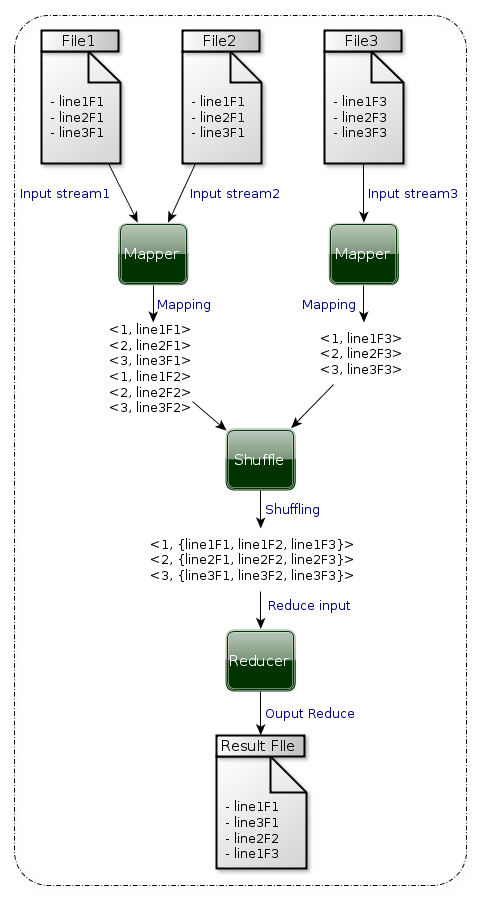
\includegraphics[width=210px,height=400px]{img/sampleProcess.png}
	\caption{Map and Reduce random sample process}\label{fig:sampleProcess}
\end{figure}

The map function is described by algorithm~\ref{alg:map}. Before presenting the
algorithm, some previous definitions are necessary. Let us denote {\it F} the set
of files stored on the cluster, {\it f} a file belonging to {\it F}, {\it l} current
line of {\it f} and {\it o} the order of the {\it L} in {\it F}.

\begin{algorithm}
		\caption{Map function for data sample \label{alg:map}}

        \SetKwInOut{Input}{Input}
        \SetKwInOut{Output}{Output}
		\Input{$F$ file set in the cluster}
        \Output{$map<Integer, String>$ 	resultant list of key-value}

		$map \leftarrow  \{\}$

		\For{\textbf{each} $f \in F$} {

			$l \leftarrow f.getNextLine()$

	    	$o \leftarrow l.getOrder()$ 

			$map.put$($o$, $l$)

		}
		
        \Return{$map$}
\end{algorithm}


The map function consists in classifying each {\it L} in the {\it F} with
it respective order {\it o}. Then intermediate key-value pair \tuple{o, l}
are emitted. Next, each pair is added to a map structure that is the output of
the map function. After the shuffle phase aggregates values sharing the same key.
These aggregated values are the input for reduce function.

\begin{algorithm}
		\caption{Reduce function for data sample \label{alg:reduce}}

        \SetKwInOut{Input}{Input}
        \SetKwInOut{Output}{Output}
		\Input{$mapList<key, values>$ list of key-values aggregated by shuffle phase}
        \Output{$list$ of selected values}

		\For{\textbf{each} $key \in mapList$} {

			\For{\textbf{each} $v \in values$} {
				$rand \leftarrow random(1, n)$

				\If{$rand \leq n$} {
					$list.add(v)$
				}

			}

		}

        \Return{$list$}
\end{algorithm}

The reduce function is in charge of the sampling and is described by algorithm~\ref{alg:reduce}.
Before presenting the algorithm, some previous definitions are necessary. Let us
denote {\it mapList} the intermediate set generated by map phase and aggregated
for the shuffle phase, it contains tuples \tuple{key, list<values>}. The {\it key}
is a key belonging to the {\it mapList}, and {\it values} is a set of values sharing
the same key. The {\it v} is a value belonging to {\it values} and {\it n} is
the amount of the values sharing the same key.

First the reduce algorithm iterates in each {\it key} and get the {\it values}
list. Then for each value {\it v} that share the same key, one random number
between the 1 and {\it n} is chosen. If the random number is lower or equal toz
{\it n} then {\it v} is added to resultant list. 
